\documentclass{article}\usepackage[]{graphicx}\usepackage[]{color}
%% maxwidth is the original width if it is less than linewidth
%% otherwise use linewidth (to make sure the graphics do not exceed the margin)
\makeatletter
\def\maxwidth{ %
  \ifdim\Gin@nat@width>\linewidth
    \linewidth
  \else
    \Gin@nat@width
  \fi
}
\makeatother

\definecolor{fgcolor}{rgb}{0.345, 0.345, 0.345}
\newcommand{\hlnum}[1]{\textcolor[rgb]{0.686,0.059,0.569}{#1}}%
\newcommand{\hlstr}[1]{\textcolor[rgb]{0.192,0.494,0.8}{#1}}%
\newcommand{\hlcom}[1]{\textcolor[rgb]{0.678,0.584,0.686}{\textit{#1}}}%
\newcommand{\hlopt}[1]{\textcolor[rgb]{0,0,0}{#1}}%
\newcommand{\hlstd}[1]{\textcolor[rgb]{0.345,0.345,0.345}{#1}}%
\newcommand{\hlkwa}[1]{\textcolor[rgb]{0.161,0.373,0.58}{\textbf{#1}}}%
\newcommand{\hlkwb}[1]{\textcolor[rgb]{0.69,0.353,0.396}{#1}}%
\newcommand{\hlkwc}[1]{\textcolor[rgb]{0.333,0.667,0.333}{#1}}%
\newcommand{\hlkwd}[1]{\textcolor[rgb]{0.737,0.353,0.396}{\textbf{#1}}}%
\let\hlipl\hlkwb

\usepackage{framed}
\makeatletter
\newenvironment{kframe}{%
 \def\at@end@of@kframe{}%
 \ifinner\ifhmode%
  \def\at@end@of@kframe{\end{minipage}}%
  \begin{minipage}{\columnwidth}%
 \fi\fi%
 \def\FrameCommand##1{\hskip\@totalleftmargin \hskip-\fboxsep
 \colorbox{shadecolor}{##1}\hskip-\fboxsep
     % There is no \\@totalrightmargin, so:
     \hskip-\linewidth \hskip-\@totalleftmargin \hskip\columnwidth}%
 \MakeFramed {\advance\hsize-\width
   \@totalleftmargin\z@ \linewidth\hsize
   \@setminipage}}%
 {\par\unskip\endMakeFramed%
 \at@end@of@kframe}
\makeatother

\definecolor{shadecolor}{rgb}{.97, .97, .97}
\definecolor{messagecolor}{rgb}{0, 0, 0}
\definecolor{warningcolor}{rgb}{1, 0, 1}
\definecolor{errorcolor}{rgb}{1, 0, 0}
\newenvironment{knitrout}{}{} % an empty environment to be redefined in TeX

\usepackage{alltt}
\usepackage[colorlinks=true, linkcolor=blue, citecolor=blue]{hyperref}
\usepackage[backend=bibtex,backref=true,hyperref=true]{biblatex}
\addbibresource{proportionality.bib}
\usepackage{amsmath}
\usepackage{amssymb}
\usepackage{bbm}
\usepackage{fullpage}
\usepackage{setspace}

\usepackage{amsthm}
 
\theoremstyle{definition}
\newtheorem{definition}{Definition}

\doublespacing

\title{RNA-Seq as a Measure of Relative Abundance: oportunities afforded by a compositional analysis framework.}
\author{Dominic LaRoche \and Dean Billheimer \and Shripad Sinari \and Kurt Michels \and  Bonnie LaFleur}
\IfFileExists{upquote.sty}{\usepackage{upquote}}{}
\begin{document}

\maketitle

\doublespacing
% \section{Abstract}


\section{Introduction}

%-- Introduce the problem and motivate the research -->
The rapid rise in the use of RNA sequencing technology (RNA-seq) for scientific discovery has led to its consideration as a clinical diagnostic tool.  However, as a new technology the analytical accuracy and reproducibility of RNA-seq must be established before it can realize its full clinical utility~\cite{SEQC/MAQC-IIIConsortium2014,VanKeuren-Jensen2014}. Recent studies evaluating RNA-seq have found generally high intra-platform and inter-platform congruence across multiple laboratories~\cite{Li2013, tHoen2013, SEQC/MAQC-IIIConsortium2014}.  Despite these promising results, there is still a need to establish reliable diagnostics, quality control metrics and improve the reproducibility of RNA-seq data.  Understanding, and capatilizing on, the relative frequency nature of RNA-Seq data provides tools for identifying batch effects, creating quality control metrics, and improving reproducibility.\\

%Targeted sequencing vs traditional sequencing 
This research is focused on developing diagnostics for targeted RNA-Seq.  Targeted sequencing allows researchers to efficiently measure transcripts of interest for a particular disease by focusing sequencing efforts on a select subset of transcript targets.  Targeted sequencing offers several benefits over traditional whole-transciptome RNA-Seq for clinical use including the elminiation of amplification bias, reduced sequencing cost, and a simplified bioinformatics workflow.  However, traditional RNA-Seq and targeted RNA-Seq data share many of the same properties so the methods described here should be easily extensible to traditional RNA-Seq.\\

%Accurately identifying batch effects, and differentiating these from true biological differences, will be necessary if smaller laboratories wish to utilize RNA-seq technology for clinical applications (cite).  Moreover, the reliable identification and removal of poor quality data produced by RNA-seq pipelines has the potential to dramatically improve the analytical accuracy and reproducibility of RNA-seq data, thereby improving its clinical utility.\\

%-- Brief intro to compositional data
Targeted and whole transcriptome RNA-Seq data provide relative frequencies of the measured transcripts.  Relative frequency measures are characterized as a vector of proportions of some whole.  These proportions are necessarily positive and sum to a constant which is determined by the measurement system and not the measurand.  For example, as an experiment, we take a large bag of marbles of different colors and pour them over a shallow bowl.  The bag holds many more marbles than the bowl so most of the marbles spill out and remain unmeasured.  Since we measure an unknown portion of the marbles in the bag we cannot know the total number of each marble color that was contained in the bag.  However, we can estimate the relative frequencies of each marble color in the bag.  The total number of marbles we observe is a function of the measurement, i.e. the size of the bowl.\\

%we count the number and type of cars passing by us in the first lane of a busy highway for 5 minutes.  We cannot observe the other lanes because they are obstructed by the first lane and we do not know haw many lanes the highway contains.  If we assume the first lane is representative of the other lanes we might be able to say something about the relative frequency of each car type on the highway, but without knowing the total number of lanes we won't be able to say anything about the total number of each car type travelling on that highway during the 5 minutes we observed. If we are able to observe 2 lanes our total number of cars observed will be greater than (or equal to) the total number of cars we observed in 1 lane.  Clearly, the total number of cars we observe is a function of the measurement process and not the total number of cars on the highway.\\

%Suppose we repeat this experiment several times.  Since we can only observe a finite number of cars during a 5 minute span , if any 1 car type increases in frequency then the other car types must then decrease in frequency proportionally.  This proportionality is strictly enforced if the lane is at maximum capacity, but one can imagine if the number of cars observed is very small compared to the number of cars possible to observe the proportionality may be less strict.  \\

Suppose we repeat this experiment a second time with a new bag of marbles to which we add a bunch of red marbles.  Since the bowl is fixed in size, if capture more rd marbles in the bowl (as we expect) then the other colors int he bowl must then decrease in frequency proportionally even if the absolute number of the other colors remains constant.  This proportionality is strictly enforced when the bowl is small and the bag is large, but one can imagine a scenario where the bowl is large and the bag is small in which the propotionality is somewhat relaxed.\\

%-- Short description of compositional data and justification of treating RNA-seq as compositional-->

Similarly, NGS-based RNA-Seq methods are also relative frequencies.  High-throughput RNA-Seq instruments have a maximum number of reads available per run.  For example, the Roche 454 GS Junior \textsuperscript{(TM)} claims approximately 100,000 reads per run for shotgun sequencing and 70,000 reads per run for amplicon sequencing.  The Illumina Mi-Seq, with shorter read lengths, is limited to 25 million reads per sequencing run.  These reads are distributed across all of the samples included in a sequencing run and, therefore, impose a total sum constraint on the data.  This constraint cascades down to each probe or tag within a sample which is, in turn, constrained by the total number of reads allocated to the sample thereby creating a natural hierarchical structure to RNA-Seq data.\\

Previous authors have identified the relative nature of RNA-Seq data~\cite{Robinson2007, Anders2010, Robinson2010, Law2014, Lovell2015}.  For example, Robinson and Smyth (2007)~\cite{Robinson2007} consider counts of RNA tags as relative abundances in their development of a model for estimating differential gene expression implemented in the Bioconductor package edgeR.  Similarly, Robinson and Oshlack (2010) explicitly acknowledge the mapped-read constraint when developing their widely used Trimmed-Mean of M-values (TMM) normalization method for RNA-Seq data.  \\%However, none of these authors reference the large body of literature on the analysis of compositions.


The positivity and summation constraint complicate the analysis of relative frequency data.  John Aitchison observed that relative frequency data is compositional and developed a methodology based on the geometric constraints of composiitons~\cite{Aitchison1986}.  As early as 1896 Karl Pearson~\cite{Pearson1896} identified the spurious correlation problem associated with compositions.  Aitchison (1986)~\cite{Aitchison1986} identified the difficulty of interpreting the covariance matrix of a composition.  Recent authors have argued that ignoring the sum constraint can lead to unexpected results and erroneous inference~\cite{Lovell2011}.  Despite the evidence that RNA-Seq data are compositional in nature, few researchers have extended the broad set of compositional data analysis theory and operations for use in RNA-Seq analysis problems.  We provide a brief background on compositional methods.  We then extend existing compositional data methodology to include 3 (?) quality control metrics for RNA-Seq data. Finally, we show how compositional properties can be exploited to facilitate exploratortion of high-dimensional RNA-Seq data.\\

%-- Describe sequencing QC metrics a little
Illumina incorporates several sequencing specific quality control metrics including percentage of clusters passing filters and cluster density analysis. Other quality control metrics are also available, such as HTQC~\cite{Yang2013}.  However, most of the quality control metrics, while informative, are subjective...  %not sure what to say about these

Extraction-free sequencing technologies, such as HTG EdgeSeq, permit the use of very small sample volumes but create the need for additional quality control metrics since poor quality samples, which would likely be removed after unsucessful RNA extraction in extraction-based technologies, can be sequenced.\\ %this needs a lot of work!

\section{Methods}

\subsection{Compositional Data}
%-- CODA intro -->
We begin with a brief introduction to compositional data, its properties, and some established analytical methods.  Compositional data is defined as any data in which all elements are non-negative and sum to a fixed constant~\cite{Aitchison1986}. %-- Establish notation  and data hierarchy-->
For RNA-seq data, the total sum constraint is imposed by the limited number of available reads in each sequencing run.  Since this total differs between sequencing platforms we will refer to the total number of available reads as $\mathbb{T}$. These reads are distributed among the $D$ samples in a sequencing run such that:
\begin{equation}
\sum_{i=1}^{D} t_i = \mathbb{T}
\label{sumt}
\end{equation}
where $t_i$ represents the total reads for sample $i$.  Because of the total sum constraint, the vector $\mathbf{t}$ is completely determined by $D-1$ elements since the $D^{th}$ element of $\mathbf{t}$ can be determined from the other $d = D-1$ elements and the total $\mathbb{T}$:  
\begin{equation}
t_D = \mathbb{T} - \sum_{i=1}^{d} \mathbf{t_i}
\label{sumConst}
\end{equation}
In \ref{sumConst}, any of the elements can be chosen for $t_D$ with the remaining elements labeled $1, ..., d$ in any order~\cite{Aitchison1986}.  Similarly, the total reads for each sample ($t_i$) are distributed among the $P$ transcript targets in the assay such that $\sum_{j=1}^{P} p_{ij} = t_i$, where $p_{ij}$ is the total reads allocated to target $j$ in sample $i$.  We highlight the hierarchichal structure of RNA-Seq data as it leads to useful properties when devloping quality control metrics.\\


From equations~\ref{sumt} and~\ref{sumConst} it is clear that the total reads allocated to each of the $D$ samples represent a $D - 1 = d$ dimensional simplex ($\mathcal{S}^d$). This leads to a diffculty in interpreting the traditional $D \times D$ covariance structure.  In particular, it is clear that for a D-part composition $\mathbf{x}$, $\text{cov}(x_1, x_1+ \cdots +x_D) = 0$  since $x_1 + \cdots + x_D$ is a constant.  Moreover, the sum constraint induces negativity in the covariance matrix,

\begin{equation}
\text{cov}(x_1, x_2) + \cdots + \text{cov}(x_1, x_D) = -\text{var}(x_1).
\label{negbias}
\end{equation}

Equation~\ref{negbias} shows that at least one element of each row of the covariance matrix must be negative. Aitchison refers to this as the "negative bias difficulty" (although `bias' is not used in the traditional sense;~\cite{Aitchison1986}, p. 53). The existence of these negative values creates problems for the interpretation of the covariance matrix since values are no longer free to range between 0 and 1.\\


Because of the difficulties outlined above, standard statistical methodology is not always appropriate~\cite{Aitchison1986} and can produce misleading results~\cite{Lovell2015}.  To overcome these obstacles, Aitchison~\cite{Aitchison1980} proposed working in ratios of components. We focus on the Centered Log-Ratio (CLR) which treats the parts of the composition symmetrically and provides an informative covariance structure.  The CLR transformation is defined for a $D$-part composition $\mathbf{x}$ as:
\begin{equation}
y_i  = \text{CLR}(x_i) = log \left(\frac{x_i}{g(\mathbf{x})} \right),
\label{clr}
\end{equation}
where $g(\mathbf{x})$ is the geometric mean of $\mathbf{x}$.  The $D \times D$ covariance matrix is then defined as:
\begin{equation}
\Gamma = \left[\text{cov}\left(y_i, y_j \right): i,\ j = 1, ..., D \right]
\label{gamma}
\end{equation}
\\

To avoid numerical difficulties arising from sequence targets with 0 reads Martin-Fernandez et al.~\cite{Martin-Fernandez2000} an additive-multiplicative hybrid transformation.  This transformation is additive on the zero components but multiplicative on the non-zero components.  It has several advantages over the simple additive transformation since it preserves several important compositional properties.  Martin-Fernandez et al.~\cite{Martin-Fernandez2000} recommend using 0.55 $\times$ the smallest detectable value as originally suggested by Sandford et al.~\cite{Kiers2000, Sanford1993}. The threshold value for RNA-seq data must account for read depth since a 0 in a sample with a library size of 1 thousand reads would potentially not be 0 if the total number of reads was increased to 1 million.  Therefore, we define the threshold value for a sample as $\delta = \frac{0.55}{\text{Total Reads}}$.  The Martin-Fernandez transformation then becomes,

\begin{equation}
v_i = \frac{x_i}{\sum_{i = 1}^{D} x_i}
\end{equation}

\begin{equation}
u_i  = 
  \begin{cases} 
    \delta  & \text{ if }v_i = 0\\
    v_i \times \left[1 - \left( \sum_{i = 1}^{D} \mathcal{I}_{\left(v_i = 0\right)}\right) \times \delta  \right] & \text{ if }x_i \ne 0.\\
  \end{cases}
\label{MFclr}
\end{equation}

The CLR transformation is then applied to the vector $\mathbf{u}$.\\

The CLR transformation can be viewed as an extension of the familiar Counts per Million (CPM) transformation~\cite{Law2014} defined as, $log_2 \left(\frac{r_{gi}+0.5}{t_i+1} \times 10^6 \right)$, where $r_{gi}$ is the number of sequence reads for each probe ($g$) and sample ($i$), (scaled to avoid zero counts), adjusted for the number of mapped reads (library count) for each sample $t_i$ (scaled by a constant 1 to ensure the proportional read to library size ratio is greater than zero). The primary difference between the CLR and log(CPM) transformations is in the use of the geomtric mean in the denominator of the CLR transformation. Although the CLR transformation preserves the original dimmension of the data, and gives equal treatment to every element of $\mathbf{x}$, the resulting covariance matrix, $\Gamma$, is singular.  Therefore, care should be taken when using general multivariate methods on CLR transformed data.\\

Similarly, the compositional geometry must be accounted for when measuring the distance between two compositions or finding the center of a group of compositions~\cite{Aitchison2000}.  Aitchison~\cite{Aitchison1992} outlined several properties for any compositional difference metric which must be met: scale invariance, permutation invariance, perturbation invariance (similar to translation invariance for Euclidean distance), and subcompositional dominance (similar to subspace dominance of Euclidean distance).  The scale invariance requirement is ignorable if the difference metric is applied to data on the same scale (which is generally not satisfied in raw RNA-seq data due to differences in read depth). The permutation invariance is generally satisfied by existing methods such as Euclidean distance~\cite{Martin-Fernandez1998}. However, the perturbation invariance and subcompositional dominance are not generally satisfied~\cite{Martin-Fernandez1998}. \\

Aitchison~\cite{Aitchison1986, Aitchison1992} suggests using the sum of squares of all log-ratio differences.  Billheimer, Guttorp, and Fagan~\cite{Billheimer2001} use the geometry of compositions to define a norm which, along with the perturbation operator defined by Aitchison~\cite{Aitchison1986}, allow the interpretation of differences in compositions. Martin-Fernandez et al.~\cite{Martin-Fernandez1998} showed that applying either Euclidean distance or Mahalanobis distance metric to CLR transformed data satisfies all the requirements of a compositional distance metric. Euclidean distance on CLR transformed compositions is referred to as Aitchison distance:

$$d_A(x_i, x_j) = \left[\sum_{k=1}^D \left( log \left(\frac{x_{ik}}{g(x_i)} \right) - log \left(\frac{x_{jk}}{g(x_j)} \right) \right)^2  \right]^\frac{1}{2}$$

or 

$$d_A(x_i, x_j) = \left[\sum_{k=1}^D \left( clr(x_{ik}) - clr(x_{jk}) \right)^2  \right]^\frac{1}{2}.$$
\\

Up to this point we have referred to the total reads available per sequencing run, $\mathbb{T}$.  However, it is more typical to work with the aligned reads in practice.  The total aligned reads, $T$, is always a fraction of the total reads available for a sequencing run, $\mathbb{T}$.  The fraction of the total reads aligned can be a affected by multiple factors, including the choice of alignment algorithm, which we do not address here.  We assume that $T$ imposes the same constraints on the data as oultined above for $\mathbb{T}$ and will refer exclusively to $T$ hereafter.\\  



\subsection{Sample Quality Control}
Problems with sample quality, library preparation, or sequencing may result in a low number of reads allocated to a given sample within a sequencing run.  The Percent Pass Filter (\% PF) metric provided on Illumina sequencers provides a subjective measure that can identify problems with sequencing that result in a low number of reads allocated to a sample.  However, \% PF will not necessarily catch problems associated with poor sample quality of or problems with sample pre-processing since these processes may affect cluster generation, and not just cluster quality.  Morevoer, there is currently no objective way to evaluate sample quality based on the total number of reads attributed to a sample. We propose a method for objectively identifying problematic samples based on the total number of reads allocated to the sample. \\

For most experimental designs we expect the number of reads allocated to each sample in a sequencing run to arise from the same general data generating mechanism, regardless of experimental condition.  The objective is then to determine which samples arise from a different mechanism.  Outlier detection is well suited for discovering obervations that deviate so much from other observations that they are likely to have arisen from a different mechanism~\cite{Hawkins1980}.  We base our method off Tukey's box-plots~\cite{Tukey1977}, which is a well used and robust method for detecting outliers~\cite{Ben-Gal2009}.\\

We expect the total number of reads allocated to each sample, $t_i$, to be equivalent notwithstanding random variation. For a given sequencing run with $D$ samples we define the vector of total reads allocated to each sample as $\mathbf{t}$.  Since the $D$ dimensional vector $\mathbf{t}$ is a composition we have $\mathbf{t} \in \mathcal{S}^{D-1}$, the $D-1$-dimensional simplex. As noted above, traditional statistical methods may not be appropriate for data in the simplex.  Therefore, we map $\mathbf{t} \in \mathcal{S}^{D-1} \rightarrow \mathbf{x} = CLR(\mathbf{t}) \in \mathcal{R}^D$ using the Centered Log Ratio transformation~\ref{clr}.  We then apply Tukey's method for detecting outliers to $\mathbf{x}$, which simply identifies those observations which lie outside 1.5 times the inter-quartile range.

\theoremstyle{definition}
\begin{definition}
$x_i$ is a quality control failure if $x_i <$ lower-quartile$- 1.5 \times$ IQR \emph{or}  $x_i >$ upper-quartile$+ 1.5 \times$ IQR, where IQR is the interquartile range of $\mathbf{x}$.
\end{definition}

We demonstrate the utility of our sample quality control measure using two sets of targeted RNA-Seq data: 1) 120 mRNA technical replicate universal RNA samples prepared with the HTG EdgeSeq Immuno-Oncology assay and sequenced in 5 different equally sized runs, and 2) 105 miRNA technical replicate samples of human plasma, FFPE tissue, and Brain RNA prepared with the HTG EdgeSeq Whole Transcriptome miRNA assay.  These two data sets differ in the both the type of RNA (mRNA versus miRNA) and the number of sequence targets in each assay (558 versus 2,280 targets, for the mRNA and miRNA assays respectively).  All samples were prepared for sequencing using the HTG EdgeSeq Processor and sequenced with an Illumina Mi-Seq sequencer.\\

\subsection{Batch Effects and Normalization}
Batch effects arising from differing labratory conditions or operator differences have been identified as a problem in high-throughput measurement systems~\cite{leek2010, chen2011}.  Identifying and controlling for batch effects is a critical step in the transition of RNA-Seq from the lab to the clinic.  Batch effects are typically identified with a hierarchical clustering (HC) method or principal components analysis (PCA).  For both methods, the multivariate distance between the samples is visualized. either in a biplot for PCA or a dendrogram for HC, to check for the existence of clusters of samples related to batch. % and removed through various normalization methods~\cite{Robinson2007, Anders2010, Robinson2010, Law2014, leek2014}.  \\ %I wonder if I should move that last line
The compositional nature of RNA-Seq data has important implications for the detection of batch effects because of the difficulty of interpreting the covariance matrix~\cite{Aitchison1986} and the incompatibility with standard measures of distance between compositions as noted above~\cite{Aitchison1986,Martin-Fernandez1998}.\\  %The CLR transformation facilitates both batch effect detection and normalization.  The CLR transformed covariance matrix is suitable for exploration through PCA (using biplots)~\cite{Aitchison2002} or hierarchical clustering using standard Euclidean or Mahalanobis distance~\cite{Martin-Fernandez1998}.  \\

The next generation sequencing process results in arbitrary differences in scale among samples as some samples will receive more total reads than others by chance. Principle components analysis is sensitive to differences in scale among the variables, failure to remove these difference can mask potential batch effects and leave unwanted technical variation in the data.  Most normalization methods use a scaling factor calculated for each sample to rescale the read count for each gene within the sample~\cite{Dillies2013}.  The CLR transformation can also be viewed as a scaling factor (the inverse of the geomtric mean $1/g(x)$), which is multiplied to each gene read count in the sample.\\

Aitchison demonstrated that the CLR transformation has several other useful properties in addition to rescaling the data~\cite{Aitchison1986}, particularly with respect to PCA biplots~\cite{Aitchison2002}.  Most notably for the detection of batch effects, the distance between any two points representing samples in the form-biplot approximates the Euclidean distance between the two samples.  The CLR transformation retains the property that this distance is at least as great as the distance between any corresponding subset of these two compositions (subspace dominance).  Other scaling methods do not necessarily satisfy this property when used with compositions, and therefore batch effects may be masked.\\

%toy example of distance issue when checking for batch effects here


\section{Results}

\subsection{Sample Quality Control}

We compare the utility of our method to evaluation of the untransformed total counts.  Figure~\ref{totalFig} shows a boxplot and heatmap of the total number of reads allocated to each sample in each of 5 sequencing runs.  Figure~\ref{clrFig} shows the same data after CLR transformation.  After transformation the poor samples become much more visually evident in the heat maps and the number of poor samples detected increases from 1 to 6.  \\

\begin{figure}
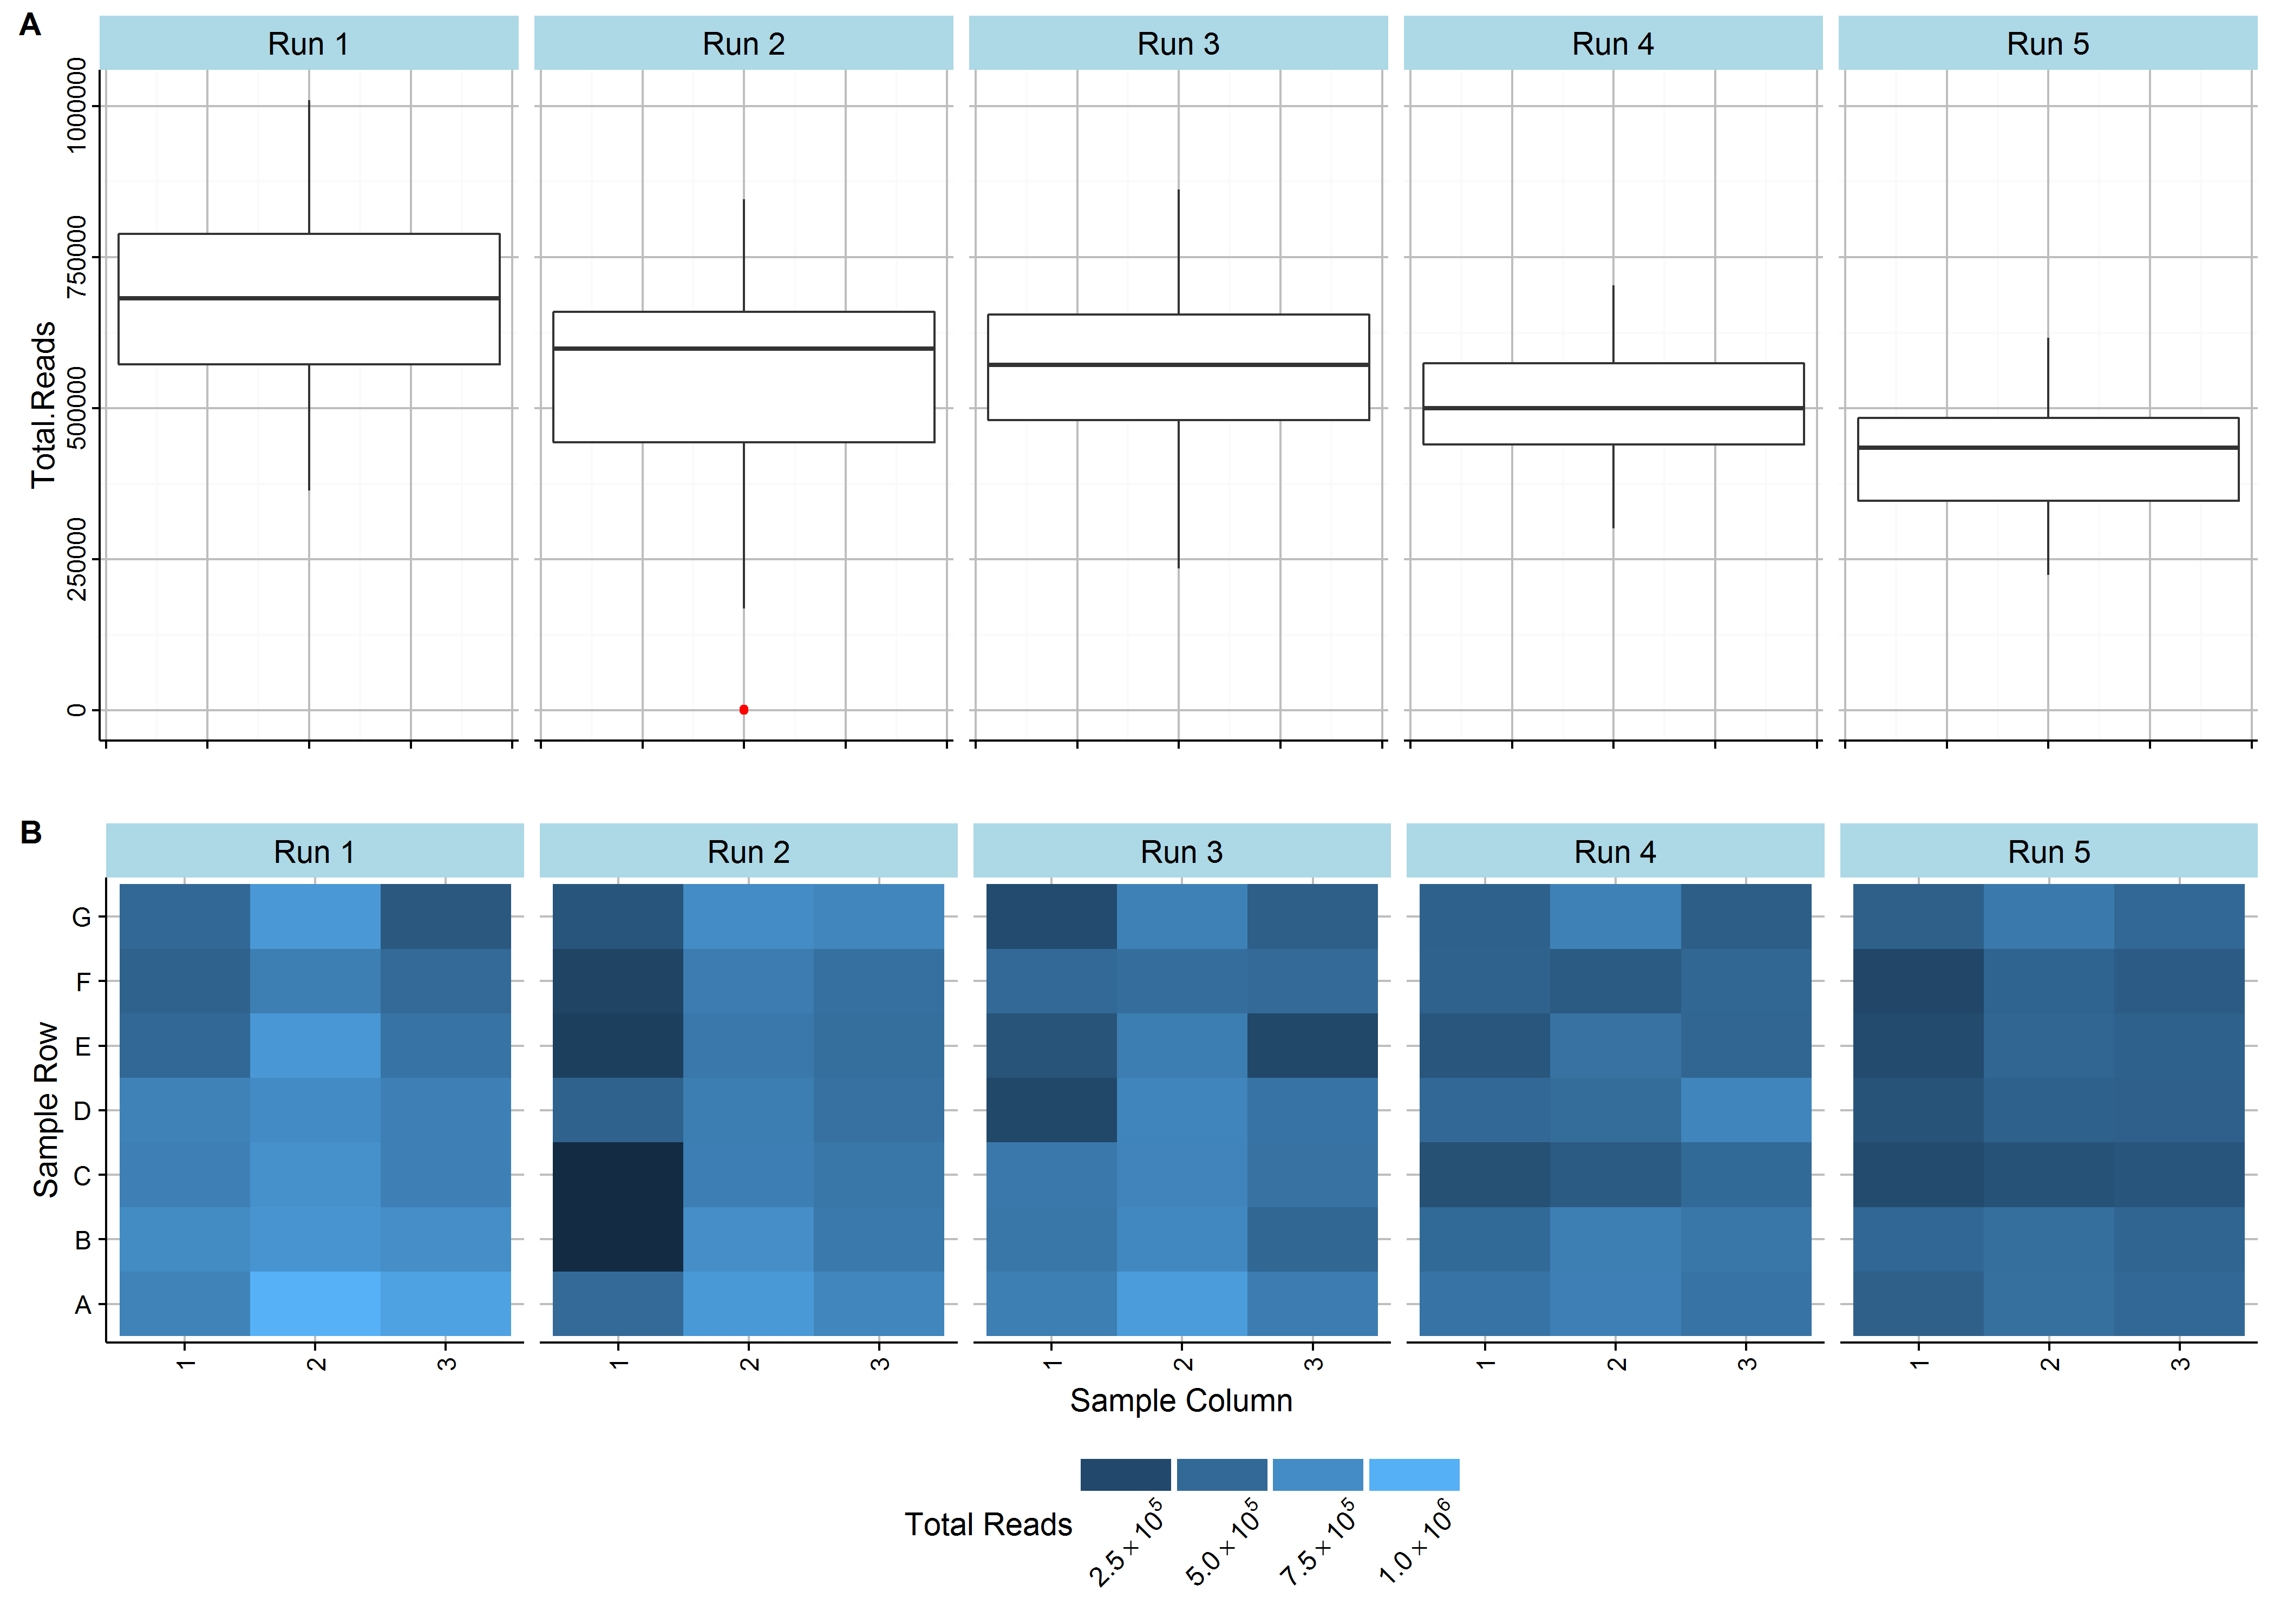
\includegraphics[scale=.5]{./Figures/IO_Repro_Combined_RawTotals}
\caption{A) Distributions of total reads allocated to each sample in 5 runs on an Illumina Mi-Seq sequencer. Only 1 sample is identified as a problematic sample. B) Heatmaps showing the relative totals for each sample within each run.  The darker heatmaps for runs 4 and 5 reflect the generally lower number of total reads in those sequencing runs as compared to runs 1 and 2.  This is caused by normal variation in the number of reads available in a sequencing run.}
\label{totalFig}
\end{figure}
 
\begin{figure}
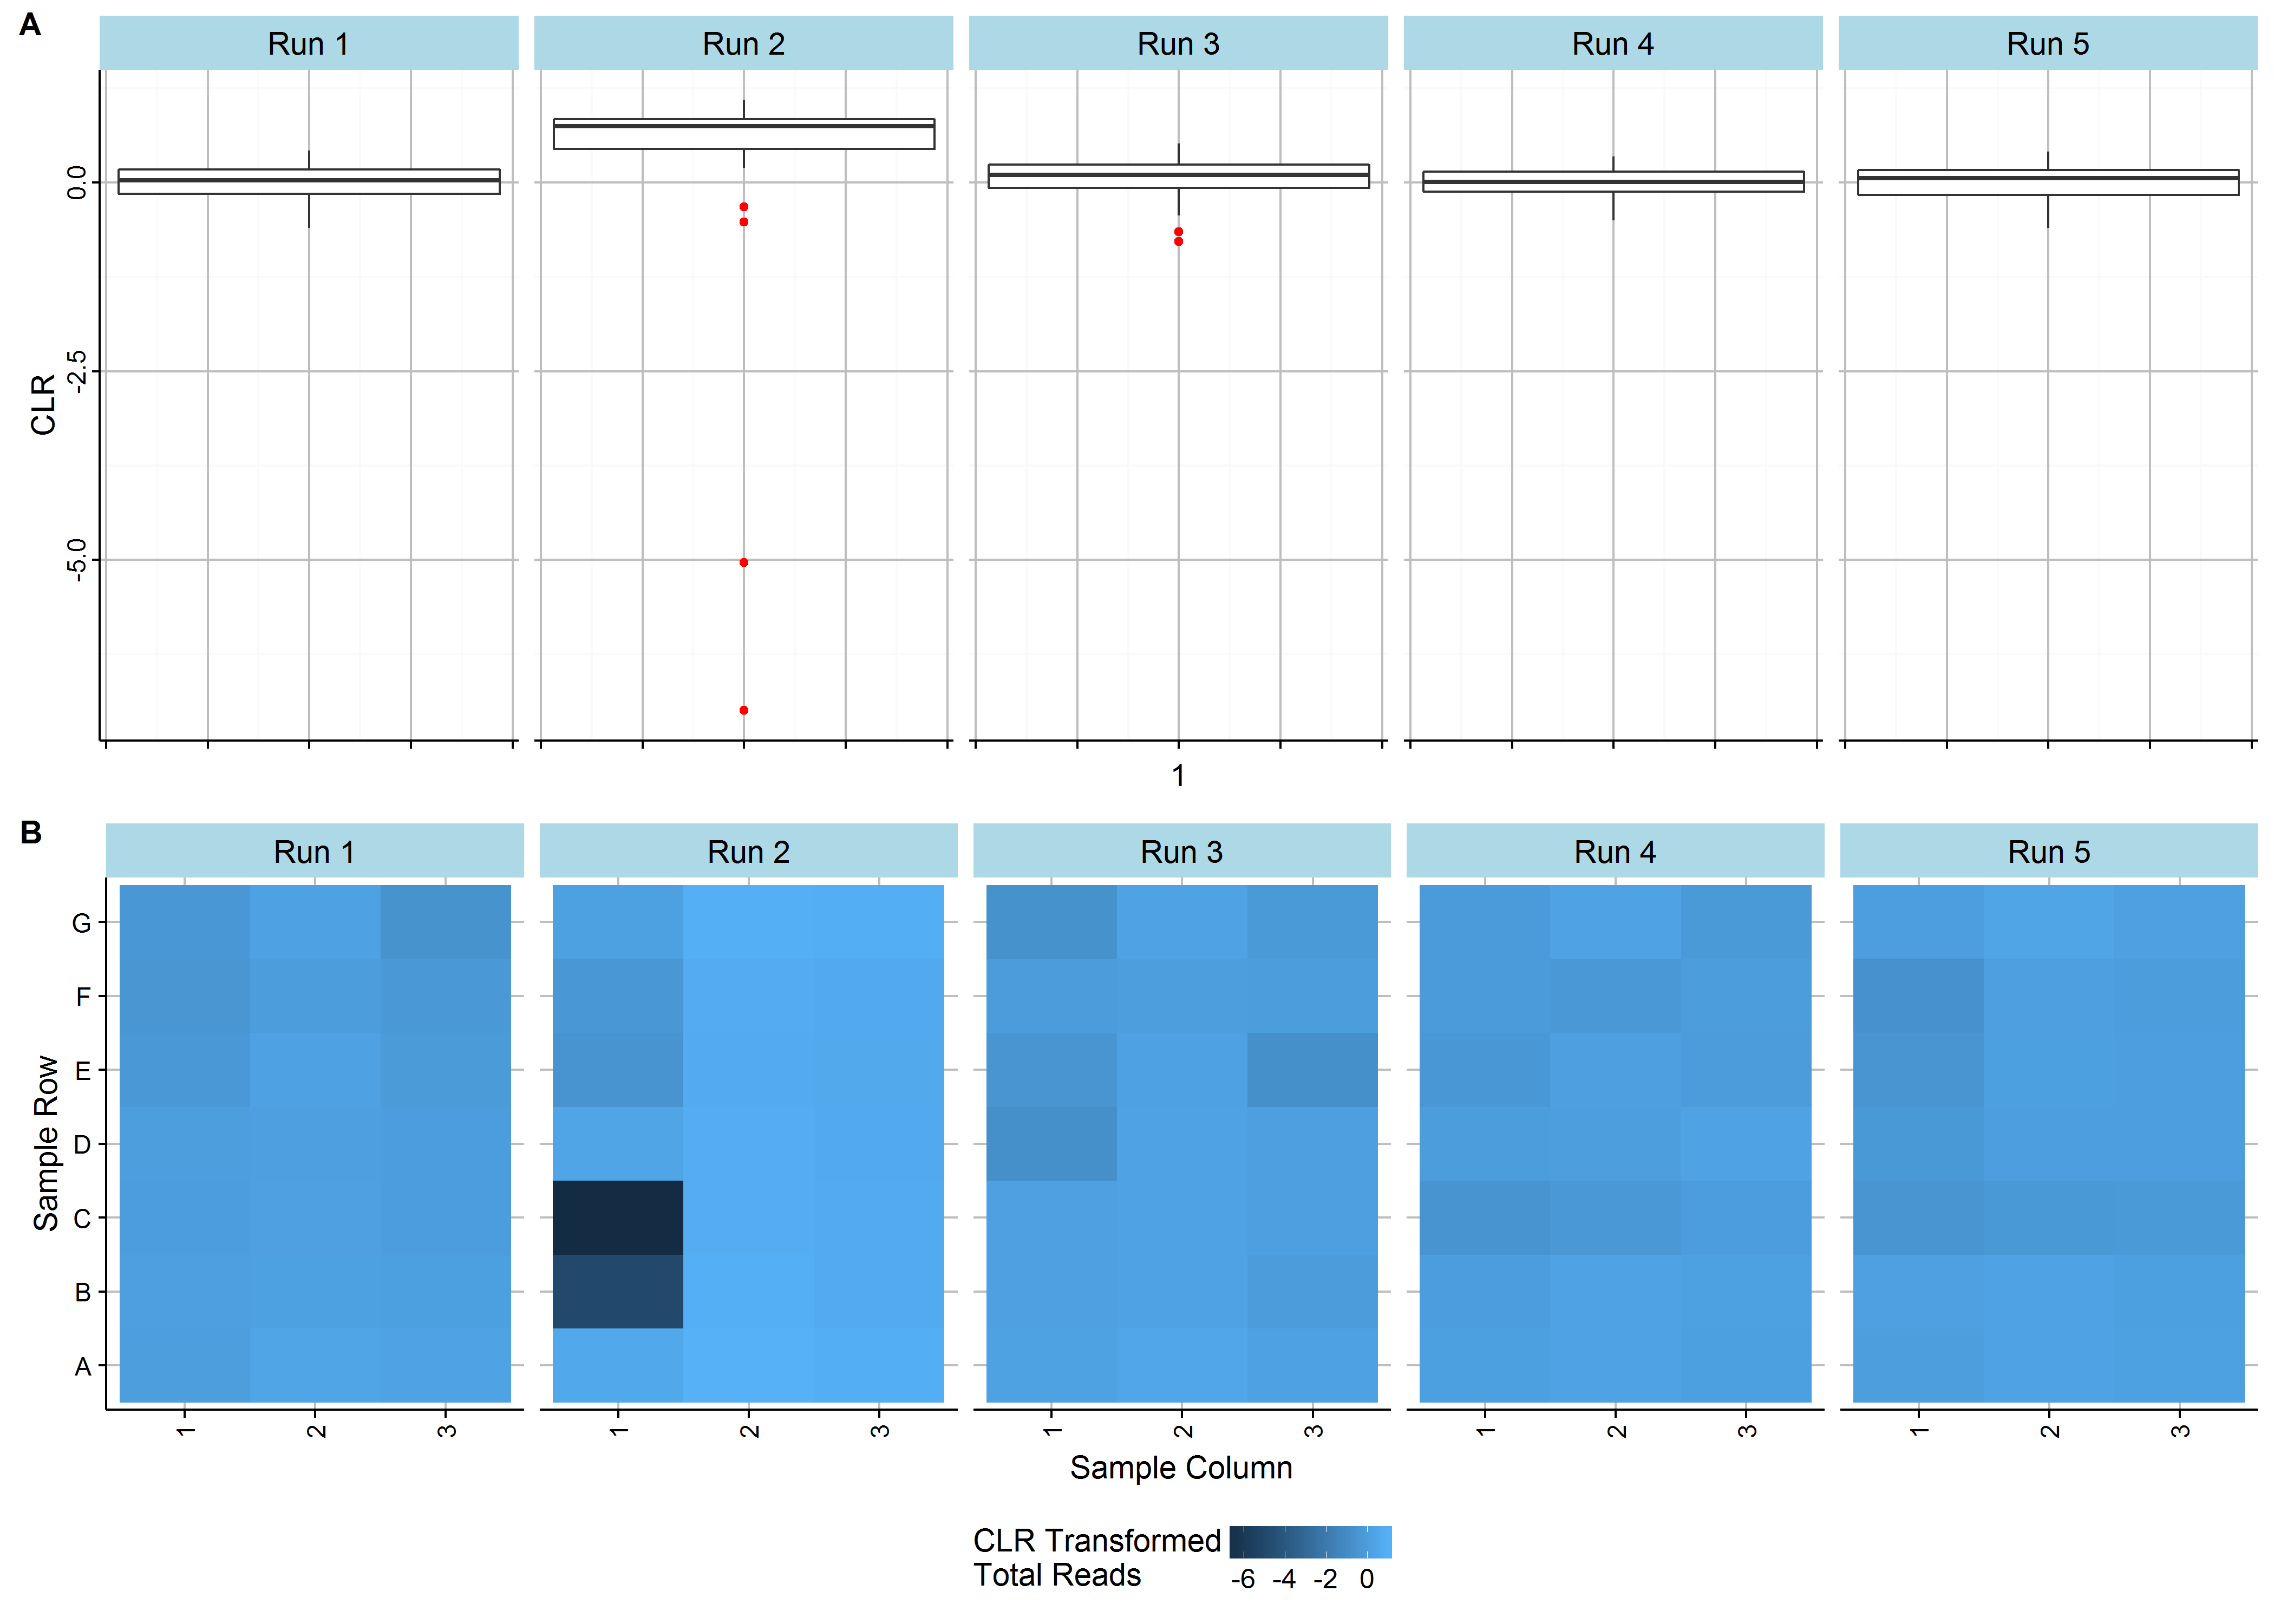
\includegraphics[scale=.5]{./Figures/IO_Repro_Combined_CLR}
\caption{A) Distributions of CLR tranformed total reads allocated to each sample in 5 runs on an Illumina Mi-Seq sequencer. After CLR transformation, 6 samples are identified as a problematic. B) Heatmaps showing the relative CLR transformed totals for each sample within each run.}
\label{clrFig}
\end{figure}

\newpage

\printbibliography

\end{document}
